%\documentclass[letterpaper, 10pt]{sigcomm-alternate}

\documentclass[peerreview, a4paper, 7pt]{IEEEtran}
%\documentclass[a4paper, 10pt]{IEEEtran}
%\documentclass{scrreprt}
\usepackage{times}
\usepackage{alltt}
\usepackage{graphicx}
\usepackage{alltt}
\usepackage{colortbl}
\usepackage[dvipsnames]{xcolor}
\usepackage{listings}


%\usepackage{color}
% \usepackage{caption2}
%\usepackage{subfigure}
%\usepackage{graphicx}
%\usepackage{colortbl}
%\usepackage[dvipsnames]{xcolor}
% \usepackage{ulem}

\usepackage{hyperref}

\pagenumbering{arabic}


%\ifx\pdfoutput\undefined
%\usepackage[pdfpagemode=none, pdfstartview=FitH, colorlinks=true, urlcolor=black, linkcolor=black, citecolor=black]{hyperref}
%\else
%\usepackage[pdftex, pdfpagemode=none, pdfstartview=FitH, colorlinks=true, urlcolor=black, linkcolor=black, citecolor=black, pdftex]{hyperref}
%\fi

\ifx\HCode\UnDef\else\hypersetup{tex4ht}\fi

%% Editorial work
% \newcommand{\purge}[1]{\textcolor{red}{\sout{#1}}}
% \newcommand{\add}[1]{\textcolor{blue}{#1}}

%%% End of editorial work.


 
\renewcommand{\em}[1]{\textit{#1}}
\begin{document}

\title{Analyzing the IETF ACE-OAuth Protocol}

\author{\authorblockN{Hannes Tschofenig\authorrefmark{1}\\}
\authorblockA{\authorrefmark{3}Arm Limited, 
Email: hannes.tschofenig@arm.com\\}
\thanks{\textsc{Position paper for the '3rd OAuth Security Workshop'~\cite{OSW2018}, x$^{th}$ and x$^{th}$ March 2018, Italy.}}
}

\date{\today}

\maketitle


\section{Abstract}

The OAuth Security Workshop series was started after a group of researchers from Trier/Germany discovered a vulnerability that was found using a formal method analysis of the protocol. While formal methods have been used to analyze Internet security protocols in the past, their use in the standardization community has not yet become common.

This article takes a recent OAuth specification, namely the ACE-OAuth framework~\cite{draft-ietf-ace-oauth-authz-09}, and uses a formal method to analyze it. The task was simplified by using available tools. Initially, Scyther~\cite{Scyther}, developed by Cas Cramer, was selected and then the results were verified with the Avispa. These tools also revealed an important aspect of usability. This memo describes the experience using a formal method analysis as well as the result of it. 

The analyzed specification lacks a description of the security goals. This makes any formal analysis difficult, since the person doing it essentially has to make an educated guess about the desired security properties. Furthermore, the Client Token protocol suffers from security flaws. At a minimum, the Client Token protocol needs to be either re-designed, or alternatively, removed from the specification.

\section{ACE-OAuth Overview}
\label{lwm2m}

The high-level architecture of ACE-OAuth is shown in Figure~\ref{ace-oauth-architecture-figure} where the OAuth Client interacts with an Authorization Server to obtain an access token. Once the OAuth Client is authenticated and authorized (potentially with the consent of the resource owner or some third party), it will receive an access token for use with a Resource Server. The Resource Server hosts the protected resource that the OAuth Client is interested in accessing. Unlike a classical OAuth bearer token, an access token used with ACE-OAuth is a proof-of-possession token, which has a key bound to it. When the OAuth Client present the access token to the Resource Server it also needs to demonstrate possession of the key associated with the access token.

ACE-OAuth was designed for use in Internet of Things (IoT) environments. As the name indicates, it uses the OAuth framework. In order to make OAuth suitable for use in IoT, it may be necessary to use CoAP instead of HTTP, DTLS instead of TLS, CBOR instead of JSON, and COSE instead of JOSE. These protocol and encoding alternatives ensure that the payloads transmitted over the air are significantly reduced in size. While such encoding details are not necessarily relevant for a formal analysis, they are useful for understanding the goal of the standardization activity in the IETF ACE working group.  

The specification~\cite{draft-ietf-ace-oauth-authz-09} supports a range of different protocol exchanges, and analyzing all of them would require a fair amount of time. 
For this reason, one exchange was focused on, namely the so-called Client Token protocol. This protocol variant was developed in order to address a very specific deployment limitation: a situation where the OAuth Client is not connected to the Authorization Server to obtain an access token. In this case, the OAuth Client needs to relay the communication via the Resource Server to the Authorization Server. This exchange is shown graphically in Figure~\ref{client-token-figure}.

\begin{figure}[!htbp]
 \centering
 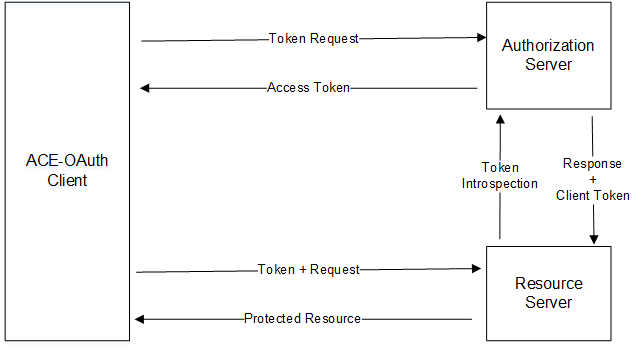
\includegraphics[scale=0.70]{ace-oauth-architecture.png}
 \caption{ACE-OAuth Architecture.}
 \label{ace-oauth-architecture-figure}
\end{figure}

As can be seen in Figure~\ref{client-token-figure}, the protocol starts with the OAuth Client sending a pre-configured access token to the Resource Server, which is then relayed to the Authorization Server via token introspection. The Authorization Server mints keying material (a session key) and conveys it to both the Resource Server and the OAuth Client. The session key is conveyed from the Authorization Server to the OAuth Client via the Client Token (hence the name Client Token protocol).

\begin{figure}[!htbp]
	\centering
	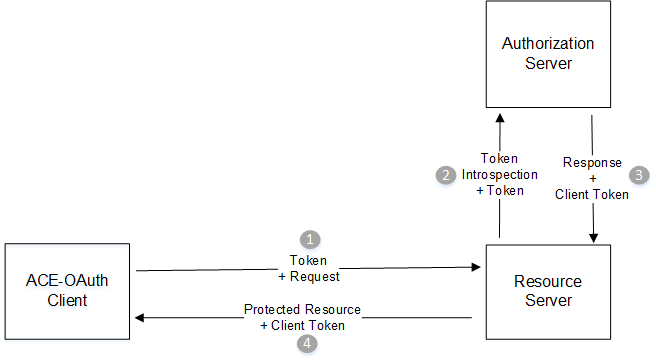
\includegraphics[scale=0.70]{client-token.png}
	\caption{Client Token Protocol.}
	\label{client-token-figure}
\end{figure}

A formal analysis requires an appropriate level of abstraction to be found. This process is essential and, if done incorrectly, may prevent one from finding a vulnerability. Before a formal analysis can be conducted, the protocol description needs to be re-written using a different notation, which will help engineers to better understand the completeness of their work.

In many cases, this step may be more insightful then the actual formal analysis itself. In the Client Token protocol analysis several assumptions were made, which are listed below: \\

\begin{description}
	\item[Pre-configured Access Token:] \hfill \\ The specification refers to a pre-configured access token that is stored by the OAuth Client and makes the following constraint: "[it] is not self-contained (i.e. it is only a reference to a token at the AS) when it is commissioned". It is essentially an identifier that allows the Authorization Server to select the appropriate key for protection of the Client Token. In the formal analysis, the assumption is that it is just an identifier referring to the OAuth Client. This pre-configured access token is transmitted in cleartext, meaning that an attacker will be able to learn it since they are able to eavesdrop into the communication. \\
	\item[Token Introspection:] \hfill \\ The specification does not mandate a specific way to protect the token introspection exchange. We assume that the communication is encrypted. \\
	\item[Proof-of-Possession:] \hfill \\ The specification does not mandate how the OAuth Client demonstrates key confirmation of the established session key with the Resource Server. Since this aspect is not relevant for the illustrated attack, we skip it. \\
	\item[Client Token Content:] \hfill \\ The specification only provides basic guidance regarding the content of the Client Token. Those basic recommendations are followed, but no additional information is included. \\ 
	\item[Key Distribution:] \hfill \\ The OAuth Client and the Resource Server share a long-term key with the Authorization Server. 
\end{description}


\section{Analysis Result}

Avispa~\cite{Avispa} and Scyther~\cite{Scyther} indicate a vulnerability in the protocol, which is caused by the lack of authentication of the OAuth Client towards the Authorization Server. This allows an adversary to act as a fake Resource Server. The scenario is not an unrealistic one, since a token is not required to have any information about the intended recipients, and the OAuth Client never expresses the intended audience in an authenticated way.

In a home or industrial environment, it is not uncommon that one Resource Server may also act as an OAuth Client in another exchange. 


Furthermore, a prominent feature of the proof-of-possession token it that it does not require OAuth Client and Resource Server information inside the token, but rather, only the proof-of-possession key. Figure~\ref{client-token-attack-figure} shows one of the attacks, graphically illustrating that the OAuth Client does not need to participate in the protocol exchange (also referred as the 'liveness property').

\begin{figure}[!htbp]
 \centering
 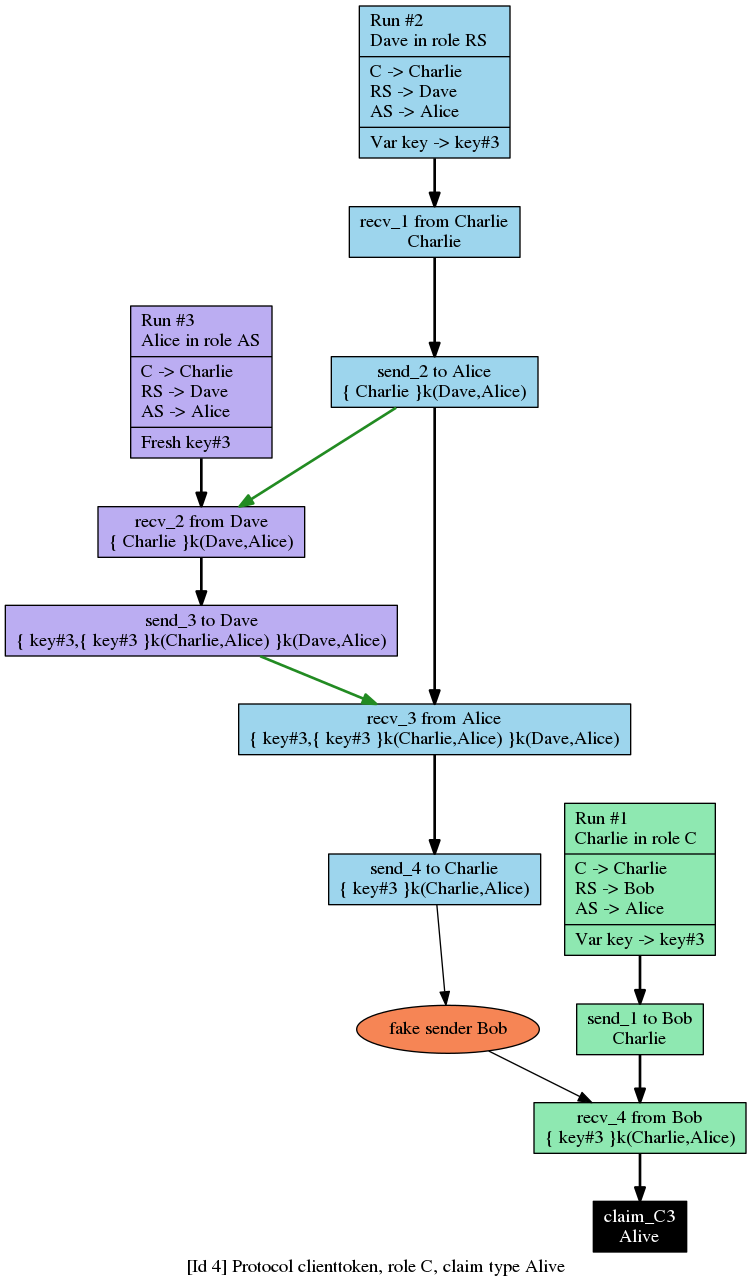
\includegraphics[scale=0.50]{client-token-attack.png}
 \caption{Attack Trace on the Client Token Protocol.}
 \label{client-token-attack-figure}
\end{figure}

The protocol exchange, which is an attack trace produced by the Scyther attack trace tool, illustrates three protocol runs (even though two would be sufficient). In the first protocol run, Charlie, acting as an OAuth Client, tries to interact with a Resource Server Bob.  Dave, acting as a rogue Resource server, provides Charlie with the Client Token obtained in another protocol run with the Authorization Server Alice. Nothing alerts Charlie that communication has been established with Dave instead of with Bob.

The Client Token protocol can be changed to mitigate against this and other attacks.This might, however, require the design of a AAA-alike protocol where an authentication protocol that runs between the OAuth Client and the Authorization Server has to be defined. This could be a single, purpose-built pre-shared key protocol or could be designed as a generic authentication framework (like the Extensible Authentication Protocol). Re-using an already specified and analyzed protocol may be the best starting point for such future work. 

\section{Summary and Recommendations}

The OAuth-ACE Client Token protocol was analyzed in response to feedback in earlier OAuth security workshops. As researchers have point out in earlier workshops, IETF specifications are often too vague to help with the analysis of security properties. While this vague nature may help one utilize the protocol in many different deployment environments, and may not even be harmful from an interoperability point of view, it leaves a large part of the security analysis to developers, who are usually not in the best position to make such an assessment.

This work, therefore, aims to create another datapoint, encouraging working groups and and specification authors to better articulate the desired security goals of IETF security specifications. 
The systematic use of formal methods by working groups will demonstrate maturity in the design process of security protocol. Formal methods allow working group participants to clearly articulate what certain protocol elements offer in terms of security (or what attacks are enabled by their omission). Formal methods, of course, do not replace the need for solid implementation, but they will help to improve the overall quality of IETF specifications.

Ideally, working groups should maintain a repository of already analyzed security protocols. This would reduce the amount of work for individual authors when defining new extensions to already existing protocols, which is what most IETF working groups do. It would allow them to analyze all protocol variants defined in a specification, since one should not just focus their attention on the main protocol variant only.

Deciding what formal method technique to use for a given task is complicated, since each tool has pros and cons. Scyther, for example, is a recently developed technique with simple syntax that is easy to use. It does, however, come with limitations in terms of what protocol properties can be analyzed. The example code in Figure~\ref{scyther-code-figure} illustrates how closely the formal description reassembles the protocol description from the specification. The Avispa tool is more powerful, but the description is verbose and more complicated to understand, as one can easily see in Figures~\ref{avispa-code-figure1} and \ref{avispa-code-figure2}. Other approaches have been used in the analysis of the OAuth / OpenID protocols, which are considerably more complex. Determining which approach is best for the analysis of IETF security protocols, where re-use and layering is a common design technique, would require further study. The level of tool support is also a criteria worthwhile to consider in such an evaluation: the Avispa tool, for example, does not appear to be supported to the same extent as more modern techniques like Scyther.


In conclusion, I believe the IETF security community would benefit from the study of formal methods, and this would help them to avoid relying so extensively on researchers. Creating awareness, for example, at the security area directorate meetings would be useful. 

\section{Acknowledgments}
I would like to thank Jennifer Andruska for her technical review of this paper and Luca Arnaboldi for his feedback. 
 
\bibliographystyle{IEEEtran}
% \bibliographystyle{acmtrans}
\bibliography{paper}

\appendix
\section{Appendix}

\begin{figure}[!htbp]
\begin{lstlisting}
usertype SessionKey;

protocol clienttoken (C,RS,AS)
{
    role C     % C: Client
    {
        var key: SessionKey; 

        send_1(C,RS, C);
        recv_4(RS,C, {key}k(C,AS) );

        claim_C1(C,Secret,key);
        claim_C3(C,Alive);
        claim_C4(C,Weakagree);
        claim_C5(C,Niagree);
        claim_C6(C,Nisynch);
    }        
    role RS     % R: Resource Server
    {
        var key: SessionKey; 

        recv_1(C,RS, C);
        send_2(RS,AS, {C}k(RS,AS)); 
        recv_3(AS,RS,  {key, {key}k(C,AS)}k(RS,AS) ); 
        send_4(RS,C, {key}k(C,AS)); 

        claim_RS1(RS,Secret,key);
        claim_RS3(RS,Alive);
        claim_RS4(RS,Weakagree);
    }    
    role AS     % A: Authorization Server
    {
        fresh key: SessionKey;

        recv_2(RS,AS, {C}k(RS,AS)); 
        send_3(AS,RS, {key, {key}k(C,AS)}k(RS,AS) ); 
    }    
}
\end{lstlisting}
\caption{Client Token Protocol in Scyther Notation.}
\label{scyther-code-figure}
\end{figure}

\begin{figure}[!htbp]
\begin{lstlisting}
% Client Token 

% C: Client
% A: Authorization Server
% R: Resource Server
 
% K_SK: key shared or intended to be shared between C and R
% Initially shared: K_CA, K_RA
	   
% Client
role client_token_C (C, A, R : agent,
                 Snd, Rcv   : channel (dy),
                 K_CA : symmetric_key)
played_by C
def=
  local State           : nat,
        K_SK            : symmetric_key

  const k_cg1, k_cg2 : protocol_id,
        sec_c_K_SK : protocol_id

  init  State := 0

  transition

  1. State = 0 /\ Rcv(start) 
       =|> State':= 1 /\ Snd(C)
  
  2. State = 1 /\ Rcv({K_SK'}_K_CA) 
         =|> State':= 2 
              /\ secret(K_SK',sec_c_K_SK,{C,R,A})		 
		 
end role 


% Resource Server
role client_token_R (R, A, C : agent,
                 Snd, Rcv : channel (dy),
                 K_RA     : symmetric_key)
played_by R
def=
  local State                 : nat,
        K_SK,K_CA             : symmetric_key

  const sec_r_K_SK : protocol_id

  init  State := 0

  transition

  1. State = 0  /\ Rcv(C') =|> 
      State':= 1 /\  Snd({C'}_K_RA)

  2. State = 1 /\ Rcv({K_SK'.{K_SK'}_K_CA}_K_RA) 
         =|> State':= 2 /\ Snd({K_SK'}_K_CA)	  
              /\ secret(K_SK',sec_r_K_SK,{C,R,A})
end role
\end{lstlisting}
\caption{Client Token Protocol in Avispa Notation (Part 1).}
\label{avispa-code-figure1}
\end{figure}

\begin{figure}[!htbp]
\begin{lstlisting}
% Authorization Server
role client_token_A (A, C, R : agent,
                 Snd, Rcv   : channel (dy),
                 K_CA, K_RA : symmetric_key)
played_by A
def=
  local State              : nat,
        K_SK            : symmetric_key

  const k_sk1, k_sk2 : protocol_id,
        sec_a_K_SK : protocol_id

  init  State := 0

  transition

   1. State = 0  /\ Rcv({C}_K_RA) =|> 
      State':= 2 /\ K_SK' := new()
              /\ Snd({K_SK'.{K_SK'}_K_CA}_K_RA) 
              /\ witness(A,C,k_sk1,K_SK')
              /\ witness(A,R,k_sk2,K_SK')
              /\ secret(K_SK',sec_a_K_SK,{A,C,R})
			  	  
end role

role session( C, A, R                             : agent,
              K_CA, K_RA                          : symmetric_key)
def=

   local CR, RC, RA, AR,ARA,RAA : channel (dy)

   composition

   client_token_C (A, C, R, CR, RC, K_CA) 
     /\ client_token_R (R, A, C , RA, AR, K_RA)
	 /\ client_token_A (A, C, R , ARA, RAA, K_CA, K_RA)


end role

role environment() def=

  const  c, a, r, i           : agent,
        kca, kra, kia      : symmetric_key

  intruder_knowledge = {c,a,r,kia}

  composition
        session(c,a,r,kca,kra)
 /\     session(i,a,r,kia,kra)
 /\     session(c,a,i,kca,kia)

end role

goal

  secrecy_of sec_a_K_SK, sec_c_K_SK, sec_r_K_SK
  authentication_on k_sk1 
  authentication_on k_sk2 

end goal
environment()
\end{lstlisting}
\caption{Client Token Protocol in Avispa Notation (Part 2).}
\label{avispa-code-figure2}
\end{figure}

\end{document}

